
%(BEGIN_QUESTION)
% Copyright 2005, Tony R. Kuphaldt, released under the Creative Commons Attribution License (v 1.0)
% This means you may do almost anything with this work of mine, so long as you give me proper credit

Shown here is the ladder logic diagram for a fire alarm system, where the activation of any alarm switch opens that (normally-closed) switch contact and sounds the alarm:

$$\includegraphics[width=15.5cm]{i02478x01.eps}$$

Write the Boolean expression for this relay circuit, then simplify that expression using DeMorgan's Theorem and draw a new relay circuit implementing the simplified expression.

Finally, analyze the two circuits and determine which one is more practical from the perspective of fail-safe.  In other words, determine which circuit will give the {\it safest} result in the event of a switch or wiring failure, and explain why.

\underbar{file i02478}
%(END_QUESTION)





%(BEGIN_ANSWER)

Original circuit expression:

$$\overline{ \overline{A} \> \overline{B} \> \overline{C} \> \overline{D} \> \overline{E} }$$

Simplified expression and circuit:

$$A + B + C + D + E$$

$$\includegraphics[width=15.5cm]{i02478x02.eps}$$

\vskip 10pt

I'll let you determine (and explain) which circuit is safest.

%(END_ANSWER)





%(BEGIN_NOTES)

Given that ``open'' switch and wiring failures are more common than ``shorted'' failures, the first circuit with the normally-closed pushbutton switches wired in series would be the safest.  In the event of an ``open'' switch failure, the alarm system will sound.  In the second circuit, an ``open'' switch failure would not trigger the alarm, and worse yet it would not work upon demand (of that one switch).

In safety instrumented systems parlance, an open switch fault in the first system leads to a ``Safe Detected'' (SD) failure, while the same fault in the second system leads to an ``Dangerous Undetected'' (DU) failure.

Here students see that even though two circuits are functionally identical (at least according to their respective Boolean expressions), they may not behave quite the same under adverse conditions (i.e. faulted switches or wiring).  This is a very important thing for them to see, because it underscores the practical need to look beyond the immediate design criteria (Boolean function) and consider other parameters (failure mode).

\vskip 20pt \vbox{\hrule \hbox{\strut \vrule{} {\bf Virtual Trip-testing} \vrule} \hrule}

This question is a good candidate for a ``Virtual Trip-testing'' exercise.  Presenting the diagram to students, you pose an assignment whereby students must figure out how to test some component of this system to check that it will operate as intended to shut down the system in an abnormal (trip) condition, with some realistic limitation (e.g. power cannot be shut off to the load).  Students then propose various methods for executing the test.  Your job is to determine whether or not their proposed tests will achieve the desired result(s).

During and after the exercise, it is good to ask students follow-up questions such as:

\begin{itemize}
\item{} Where might our planned test strategy go wrong?  In other words, what thing(s) might happen to foil our test, either to invalidate the results or to not honor the stated limitation(s)?
\item{} Suppose the limitation were different.  How would this affect our ability to carry out the test?
\item{} Is the last test strategy best one we could execute?
\end{itemize}


%INDEX% Control, fail safe: different failure modes in two different fire alarm circuits
%INDEX% Electronics review: DeMorgan's Theorem applied to ladder logic diagram

%(END_NOTES)


